% =====================================================================
%  VietForces — AI Integration Report
%
%  Compiles with EITHER XeLaTeX/LuaLaTeX OR pdfLaTeX (auto-detected below).
%  RECOMMENDED: XeLaTeX (best Vietnamese rendering).
%  On Overleaf: Menu > Compiler > XeLaTeX.
% =====================================================================
\documentclass[11pt,a4paper]{article}

% ---- engine-aware Unicode / Vietnamese setup ----
\usepackage{iftex}
\ifPDFTeX
  \usepackage[utf8]{inputenc}
  \usepackage[T5]{fontenc}   % T5 = Vietnamese encoding
  \usepackage{lmodern}
\else
  \usepackage{fontspec}      % XeLaTeX / LuaLaTeX
  \setmonofont{DejaVu Sans Mono}[Scale=0.82]
\fi

\usepackage[a4paper,margin=2.4cm]{geometry}
\usepackage{xcolor}
\usepackage{fancyvrb}
\usepackage{booktabs}
\usepackage{enumitem}
\usepackage{tikz}
\usetikzlibrary{shapes.geometric, arrows.meta, positioning, calc, fit, backgrounds}
\usepackage[hidelinks]{hyperref}
\usepackage{titlesec}

% ---- colours ----
\definecolor{vfred}{HTML}{C62828}
\definecolor{vfblue}{HTML}{1565C0}
\definecolor{vfgreen}{HTML}{2E7D32}
\definecolor{vfgray}{HTML}{555555}
\definecolor{boxbg}{HTML}{F4F4F4}
\definecolor{boxframe}{HTML}{BDBDBD}

% ---- verbatim style for prompts / JSON ----
\fvset{
  frame=single,
  framerule=0.4pt,
  rulecolor=\color{boxframe},
  fontsize=\small,
  breaklines=true,
  breakanywhere=true,
  breaksymbolleft={},
  xleftmargin=4pt,
  xrightmargin=4pt,
}

\titleformat{\section}{\Large\bfseries\color{vfred}}{\thesection}{0.6em}{}
\titleformat{\subsection}{\large\bfseries\color{vfblue}}{\thesubsection}{0.6em}{}

% ---- tikz node styles ----
\tikzset{
  layer/.style={rectangle, rounded corners=3pt, draw=vfgray, very thick,
    fill=boxbg, text width=6.2cm, align=center, minimum height=1.05cm,
    font=\small},
  cloud/.style={rectangle, rounded corners=3pt, draw=vfred, very thick,
    fill=vfred!8, text width=6.2cm, align=center, minimum height=1.05cm,
    font=\small},
  store/.style={rectangle, rounded corners=3pt, draw=vfgreen, very thick,
    fill=vfgreen!8, text width=4.2cm, align=center, minimum height=1.05cm,
    font=\small},
  flow/.style={rectangle, rounded corners=3pt, draw=vfblue, thick,
    fill=vfblue!6, text width=3.6cm, align=center, minimum height=0.85cm,
    font=\footnotesize},
  dec/.style={diamond, aspect=2, draw=vfred, thick, fill=vfred!6,
    align=center, font=\footnotesize, inner sep=1pt},
  term/.style={rectangle, rounded corners=10pt, draw=vfgreen, thick,
    fill=vfgreen!8, align=center, font=\footnotesize, minimum height=0.7cm},
  ar/.style={-{Latex[length=2.2mm]}, thick},
}

% =====================================================================
\begin{document}

\begin{titlepage}
\centering
\vspace*{2.5cm}
{\Huge\bfseries\color{vfred} VietForces\par}
\vspace{0.4cm}
{\Large A Gamified Vietnamese Learning App\par}
\vspace{0.2cm}
{\large\itshape AI Integration --- Implementation Report\par}
\vspace{1.6cm}
{\large
This report documents how the AI layer (OpenAI \texttt{gpt-4o-mini})
is integrated into VietForces: the architecture, the request/response
flow, and the full set of prompts used for each feature.\par}
\vspace{2.0cm}
\begin{tabular}{rl}
\textbf{Team:} & Bao, An, Hung Cuong \\[2pt]
\textbf{Platform:} & Android (Kotlin + Jetpack Compose) \\[2pt]
\textbf{AI model:} & OpenAI \texttt{gpt-4o-mini} \\[2pt]
\textbf{Networking:} & OkHttp + JSON (\texttt{org.json}) \\
\end{tabular}
\vfill
{\large \today\par}
\end{titlepage}

\tableofcontents
\newpage

% =====================================================================
\section{Overview}

VietForces is an offline-first Vietnamese learning app for foreigners. All
fast feedback (exact-match grading, ELO, streaks, spaced repetition) runs
\emph{locally}. The AI layer is only invoked for tasks that need flexible,
language-aware judgement, following the design rule ``grade locally first,
call AI only when necessary'' to keep the app fast and cheap.

\medskip
The AI layer powers four features:

\begin{enumerate}[leftmargin=1.4cm]
  \item \textbf{Writing grading} --- score a short paragraph and rewrite it.
  \item \textbf{Open-answer grading} --- accept near-correct typed answers
        (e.g.\ missing diacritics) by meaning, not string equality.
  \item \textbf{Mascot reactions} --- the rooster mascot says natural,
        context-aware encouragement instead of fixed strings.
  \item \textbf{Personalised learning path} --- analyse the user's stats and
        recommend what to practise next.
  \item \textbf{Roleplay conversation tutor} --- a multi-turn chat where the AI
        plays a real-life character (pho seller, Grab driver, market vendor)
        and the learner practises speaking Vietnamese.
\end{enumerate}

Every AI call returns \textbf{structured JSON} and degrades gracefully: if the
key is missing, the toggle is off, or the network fails, the app falls back to
its local logic and never crashes.

% =====================================================================
\section{System Architecture}

The AI code is split into three layers plus local storage. Screens never talk
to the network directly --- they go through \texttt{AiManager}, which owns the
prompts, parses the JSON reply into typed models, and wraps every call in an
\texttt{AiCallResult} (success / error) so the UI can show loading and fallback
states.

\begin{figure}[h]
\centering
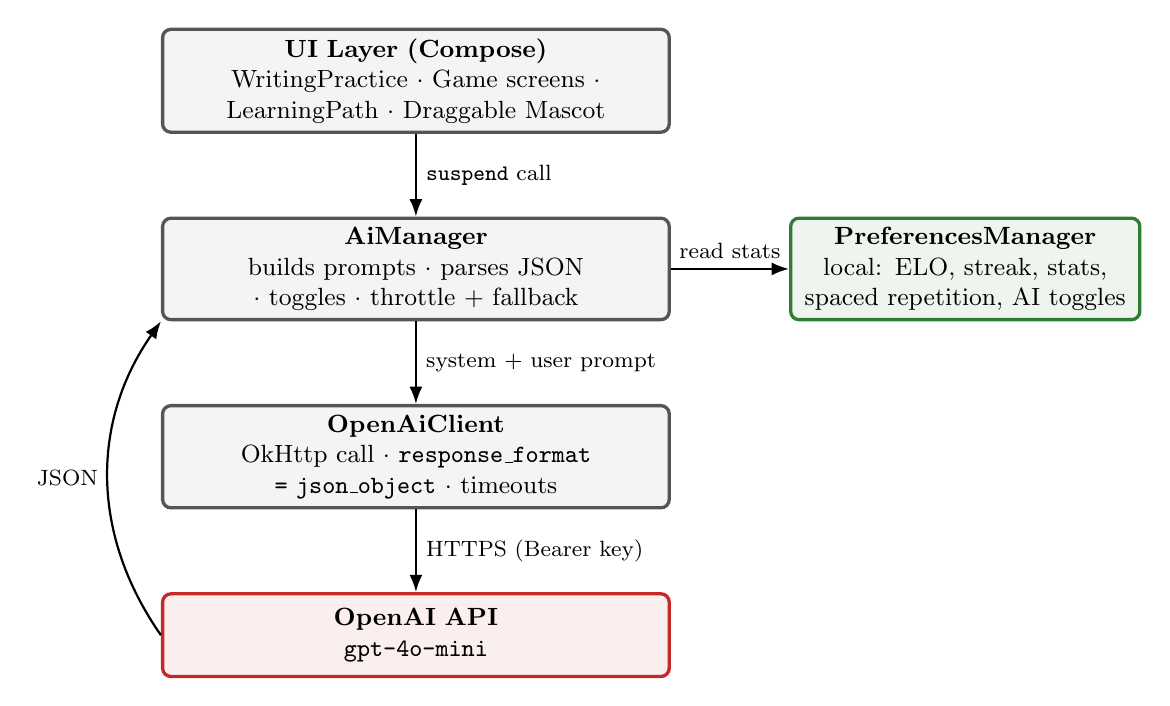
\begin{tikzpicture}[node distance=1.05cm]
  \node[layer] (ui) {\textbf{UI Layer (Compose)}\\
     WritingPractice $\cdot$ Game screens $\cdot$ LearningPath $\cdot$ Draggable Mascot};
  \node[layer, below=of ui] (mgr) {\textbf{AiManager}\\
     builds prompts $\cdot$ parses JSON $\cdot$ toggles $\cdot$ throttle + fallback};
  \node[layer, below=of mgr] (cli) {\textbf{OpenAiClient}\\
     OkHttp call $\cdot$ \texttt{response\_format = json\_object} $\cdot$ timeouts};
  \node[cloud, below=of cli] (api) {\textbf{OpenAI API}\\ \texttt{gpt-4o-mini}};
  \node[store, right=1.5cm of mgr] (store) {\textbf{PreferencesManager}\\
     local: ELO, streak, stats,\\ spaced repetition, AI toggles};

  \draw[ar] (ui)  -- node[right,font=\footnotesize]{\texttt{suspend} call} (mgr);
  \draw[ar] (mgr) -- node[right,font=\footnotesize]{system + user prompt} (cli);
  \draw[ar] (cli) -- node[right,font=\footnotesize]{HTTPS (Bearer key)} (api);
  \draw[ar] (api.west) to[bend left=35]
        node[left,font=\footnotesize]{JSON} (mgr.south west);
  \draw[ar] (mgr) -- node[above,font=\footnotesize]{read stats} (store);
\end{tikzpicture}
\caption{High-level architecture and data flow of the AI layer.}
\end{figure}

\begin{table}[h]
\centering
\small
\begin{tabular}{@{}lll@{}}
\toprule
\textbf{Component} & \textbf{File} & \textbf{Responsibility} \\
\midrule
\texttt{OpenAiClient}  & \texttt{data/remote/}      & HTTPS call: JSON mode + multi-turn chat \\
\texttt{AiManager}     & \texttt{data/manager/}     & Prompts, parsing, toggles, fallback \\
\texttt{AiModels}      & \texttt{data/model/}       & Typed results (grading, mascot, plan) \\
WritingPracticeScreen  & \texttt{ui/screens/}       & Essay input + AI feedback UI \\
LearningPathScreen     & \texttt{ui/screens/}       & Stats $\rightarrow$ AI $\rightarrow$ plan UI \\
RoleplayScreen         & \texttt{ui/screens/}       & Scenario picker + multi-turn chat \\
MascotFeedbackManager  & \texttt{ui/components/}    & Instant string + AI upgrade \\
\bottomrule
\end{tabular}
\caption{Files added / modified for the AI layer.}
\end{table}

\subsection{The HTTP request}

\texttt{OpenAiClient} sends one POST to
\texttt{https://api.openai.com/v1/chat/completions}. The key is injected at
build time from \texttt{local.properties} via \texttt{BuildConfig} (never
committed). JSON mode forces the model to reply with a single JSON object.

\begin{Verbatim}
POST /v1/chat/completions
Authorization: Bearer <OPENAI_API_KEY>
Content-Type: application/json

{
  "model": "gpt-4o-mini",
  "temperature": 0.4,
  "max_tokens": 900,
  "response_format": { "type": "json_object" },
  "messages": [
    { "role": "system", "content": "<feature prompt — see Section 4>" },
    { "role": "user",   "content": "<the content to grade / react to>" }
  ]
}
\end{Verbatim}

% =====================================================================
\section{Request Flow (local-first)}

A normal game answer is graded locally; the AI is a fallback for the hard
(typed) modes when the answer is not an exact match.

\begin{figure}[h]
\centering
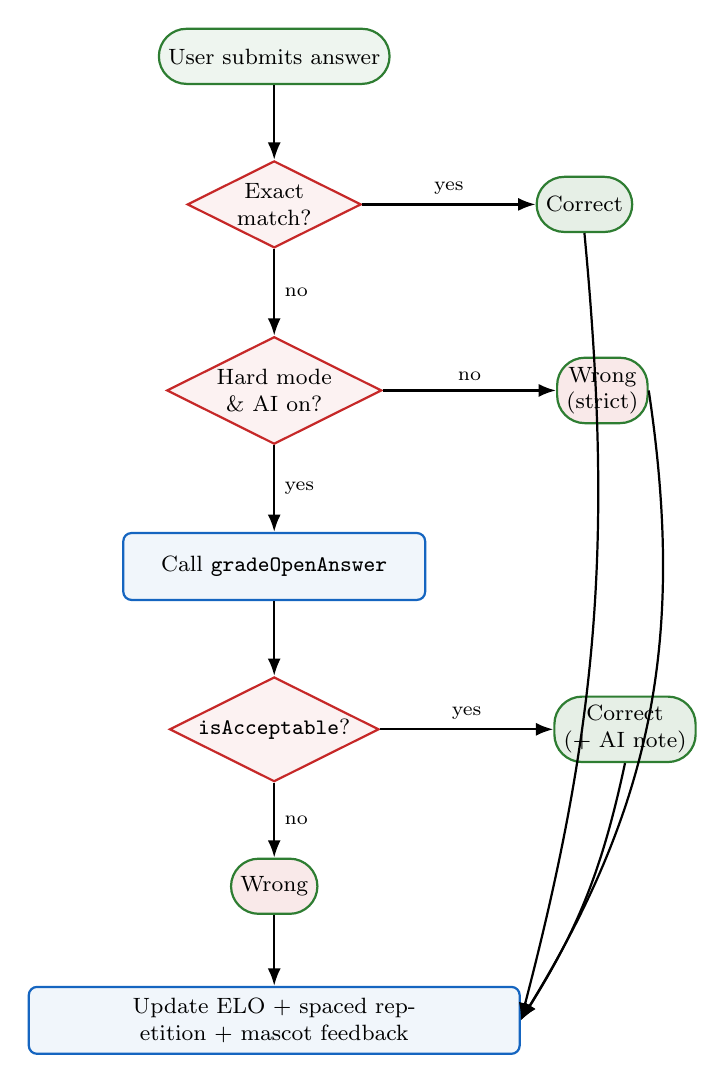
\begin{tikzpicture}[node distance=0.95cm and 1.5cm]
  \node[term] (start) {User submits answer};
  \node[dec, below=of start] (exact) {Exact\\match?};
  \node[term, right=2.2cm of exact, fill=vfgreen!12] (ok1) {Correct};
  \node[dec, below=1.1cm of exact] (hard) {Hard mode\\\& AI on?};
  \node[term, right=2.2cm of hard, fill=vfred!10] (wrong1) {Wrong\\(strict)};
  \node[flow, below=1.1cm of hard] (call) {Call \texttt{gradeOpenAnswer}};
  \node[dec, below=of call] (acc) {\texttt{isAcceptable}?};
  \node[term, right=2.2cm of acc, fill=vfgreen!12] (ok2) {Correct\\(+ AI note)};
  \node[term, below=of acc, fill=vfred!10] (wrong2) {Wrong};
  \node[flow, below=0.9cm of wrong2, text width=6cm] (upd)
       {Update ELO + spaced repetition + mascot feedback};

  \draw[ar] (start) -- (exact);
  \draw[ar] (exact) -- node[above,font=\scriptsize]{yes} (ok1);
  \draw[ar] (exact) -- node[right,font=\scriptsize]{no} (hard);
  \draw[ar] (hard)  -- node[above,font=\scriptsize]{no} (wrong1);
  \draw[ar] (hard)  -- node[right,font=\scriptsize]{yes} (call);
  \draw[ar] (call)  -- (acc);
  \draw[ar] (acc)   -- node[above,font=\scriptsize]{yes} (ok2);
  \draw[ar] (acc)   -- node[right,font=\scriptsize]{no} (wrong2);
  \draw[ar] (ok1.south)   to[bend left=10] (upd.east);
  \draw[ar] (wrong1.east) to[bend left=20] (upd.east);
  \draw[ar] (ok2.south)   to[bend left=10] (upd.east);
  \draw[ar] (wrong2) -- (upd);
\end{tikzpicture}
\caption{Local-first grading. If the network or AI is unavailable, the flow
falls back to the strict local result.}
\end{figure}

% =====================================================================
\section{Prompt History}

Each feature uses a fixed \textbf{system prompt} that defines the role and the
exact JSON shape, plus a per-call \textbf{user prompt} carrying the content.
The prompts below are reproduced verbatim from \texttt{AiManager.kt}.

% ---------------------------------------------------------------
\subsection{Writing grading (\S6.2)}
\textbf{When:} the user submits a short paragraph in Writing Practice.

\textbf{System prompt:}
\begin{Verbatim}
Bạn là giáo viên tiếng Việt thân thiện, chấm đoạn văn ngắn của người nước ngoài
đang học tiếng Việt.
Hãy đánh giá theo: ngữ pháp, dấu thanh, dấu câu, từ vựng, tính tự nhiên, đúng chủ đề,
mạch lạc.
Giọng điệu nhẹ nhàng, động viên, KHÔNG chê bai.
Chỉ trả về DUY NHẤT một JSON đúng cấu trúc sau, không thêm chữ nào ngoài JSON:
{
  "score": <số nguyên 0-10>,
  "overallFeedback": "<nhận xét chung ngắn gọn bằng tiếng Việt>",
  "mistakes": [
    {"type":"<missing_tone|punctuation|spelling|word_order|word_choice|missing_subject|other>",
     "text":"<đoạn sai>", "suggestion":"<sửa lại>", "explanation":"<giải thích ngắn>"}
  ],
  "correctedVersion": "<bản viết lại đã sửa>",
  "weaknessTags": ["<tag điểm yếu>"]
}
\end{Verbatim}

\textbf{User prompt:} \texttt{Chủ đề: "<topic>"} + the learner's paragraph.

% ---------------------------------------------------------------
\subsection{Open-answer grading (\S6.1 / \S6.3)}
\textbf{When:} hard (typed) mode and the answer is not an exact match.

\textbf{System prompt:}
\begin{Verbatim}
Bạn chấm câu trả lời tiếng Việt của người mới học. Câu trả lời của người dùng có thể
khác đáp án mẫu nhưng vẫn đúng ý (thiếu dấu, thiếu từ phụ, diễn đạt khác). Hãy đánh giá
độ tương hợp về Ý NGHĨA, không chỉ so khớp chuỗi. Giọng động viên, không chê bai.
Chỉ trả về DUY NHẤT JSON sau:
{
  "score": <0-10>,
  "isAcceptable": <true|false>,
  "feedback": "<nhận xét ngắn>",
  "mistakes": [{"type":"<...>","text":"<...>","suggestion":"<...>","explanation":"<...>"}],
  "suggestedAnswer": "<đáp án gợi ý hoặc null>",
  "weaknessTags": ["<tag>"]
}
\end{Verbatim}

\textbf{User prompt:} the question, the expected answer, and the user's answer.

% ---------------------------------------------------------------
\subsection{Mascot reaction (\S5)}
\textbf{When:} after a correct/wrong answer (throttled to once per 6 seconds).

\textbf{System prompt:}
\begin{Verbatim}
Bạn là linh vật gà trống vui vẻ đồng hành cùng người học tiếng Việt. Dựa trên ngữ cảnh
học tập, hãy nói MỘT câu ngắn (tối đa 25 từ), tích cực, động viên, có thể nhắc nhẹ lỗi.
KHÔNG chê bai.
Chỉ trả về DUY NHẤT JSON:
{"emotion":"<happy|encouraging|proud|thinking|celebrating>",
 "message":"<câu nói tiếng Việt>","shouldEncourage":<true|false>}
\end{Verbatim}

\textbf{User prompt (context), e.g.:}
\begin{Verbatim}
Người học vừa trả lời ĐÚNG. Bài nhìn hình đoán từ. Từ đúng: "mèo", người học nhập: "meo".
\end{Verbatim}

% ---------------------------------------------------------------
\subsection{Personalised learning path (\S6.4)}
\textbf{When:} the user opens the Learning Path screen (or taps refresh).

\textbf{System prompt:}
\begin{Verbatim}
Bạn phân tích dữ liệu học tiếng Việt của người dùng và tạo lộ trình học cá nhân.
Dựa trên thống kê (điểm yếu, lỗi hay gặp, chế độ làm kém), đề xuất các bài luyện ưu tiên.
recommendedMode phải thuộc: image_to_word, word_to_image, sentence_order, fill_blank,
word_chain, word_search, syllable_match, writing.
Chỉ trả về DUY NHẤT JSON:
{
  "summary":"<tóm tắt ngắn>",
  "mainWeaknesses":[{"type":"<...>","description":"<...>","recommendedPractice":"<...>"}],
  "learningPath":[{"title":"<...>","description":"<...>","targetWeakness":"<...>",
     "recommendedMode":"<...>","priority":<số 1-5>}]
}
\end{Verbatim}

\textbf{User prompt:} a generated summary of the learner's stats:
\begin{Verbatim}
Thống kê học tập của người dùng:
- Điểm ELO: 998 (hạng Nghiệp dư), streak 1 ngày.
- Tổng câu đúng: 14, sai: 6, độ chính xác: 70%.
- Độ chính xác theo chế độ:
  + Điền từ còn thiếu: 60% (6 đúng / 4 sai).
  + Nhìn hình đoán từ: 80% (8 đúng / 2 sai).
- Các mục hay sai nhất: cà phê(3 lần), bàn(2 lần).

Hãy phân tích điểm yếu và tạo lộ trình học cá nhân phù hợp.
\end{Verbatim}

% ---------------------------------------------------------------
\subsection{Roleplay conversation tutor}
\textbf{When:} the user opens a scenario in the Roleplay screen and chats.

Unlike the other features, the tutor uses \texttt{completeChat} --- a
\emph{free-form, multi-turn} call (no JSON mode). The whole conversation
(system + alternating user/assistant turns) is sent each time so the AI keeps
context and stays in character. A separate \texttt{roleplayHint} call suggests a
simple Vietnamese line the learner could say next.

\begin{table}[h]
\centering
\small
\begin{tabular}{@{}lll@{}}
\toprule
\textbf{Category} & \textbf{Scenario} & \textbf{AI plays} \\
\midrule
Food \& drink & Quán phở / Quán cà phê / Nhà hàng & seller / waiter \\
Transport     & Đi xe ôm (Grab) / Hỏi đường        & driver / passer-by \\
Shopping      & Mặc cả ở chợ / Cửa hàng quần áo    & vendor / clerk \\
Services      & Nhận phòng khách sạn / Mua thuốc   & receptionist / pharmacist \\
Social        & Làm quen bạn mới                   & a friendly local \\
\bottomrule
\end{tabular}
\caption{Roleplay scenarios, grouped by category.}
\end{table}

\textbf{System prompt (template, filled per scenario):}
\begin{Verbatim}
Bạn đang đóng vai trong một tình huống để giúp người nước ngoài luyện nói tiếng Việt.
<persona — e.g. "Bạn là cô bán phở ở Hà Nội, thân thiện và nhiệt tình...">
Hãy nói tiếng Việt TỰ NHIÊN nhưng ĐƠN GIẢN, câu NGẮN (1–2 câu), phù hợp người mới học.
Luôn giữ đúng vai, thân thiện, kiên nhẫn; dẫn dắt hội thoại và hỏi lại để khách nói tiếp.
KHÔNG chê bai. KHÔNG chuyển sang tiếng Anh trừ khi khách hoàn toàn bí.
Mục tiêu của khách trong tình huống này: <goal — e.g. "Gọi một bát phở và hỏi giá.">
\end{Verbatim}

\textbf{Example conversation (scenario ``Quán phở''):}
\begin{Verbatim}
NPC:    Em ơi vào ăn phở đi! Em muốn ăn phở bò hay phở gà?
Khách:  Cho tôi một bát phở bò
NPC:    Một bát phở bò nhé! Em có muốn thêm gì không? Như hành, chanh hay ớt?
Khách:  Bao nhiêu tiền một bát ạ?
NPC:    Một bát phở bò là 50.000 đồng. Em có muốn uống nước gì không?
\end{Verbatim}

% =====================================================================
\section{Mascot AI Flow (\S5)}

The mascot shows an instant hardcoded line for snappy UX, then \emph{upgrades}
it to an AI sentence when allowed. AI calls are throttled to avoid cost on every
answer, and the auto-hide timer resets when the AI text arrives so it has full
time on screen.

\begin{figure}[h]
\centering
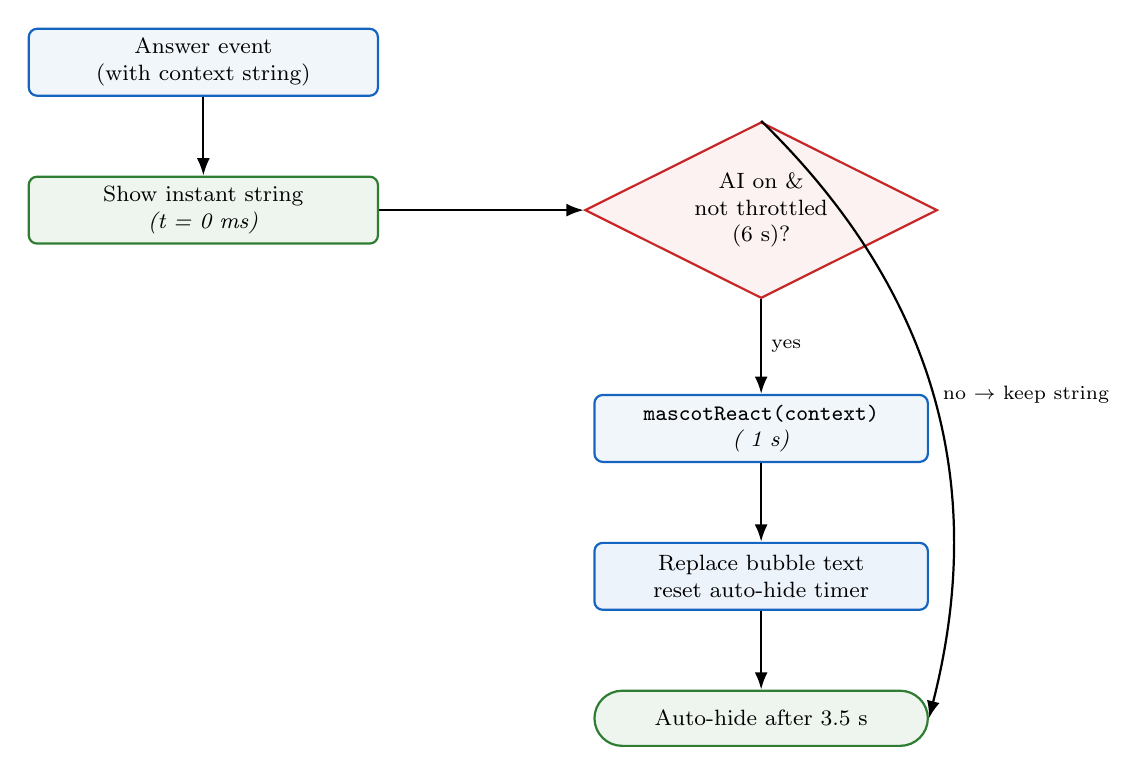
\begin{tikzpicture}[node distance=1.0cm]
  \node[flow, text width=4.2cm] (ev) {Answer event\\(with context string)};
  \node[flow, below=of ev, text width=4.2cm, fill=vfgreen!8, draw=vfgreen]
        (inst) {Show instant string\\\textit{(t = 0 ms)}};
  \node[dec, right=2.6cm of inst, text width=2.4cm]
        (gate) {AI on \&\\ not throttled\\ (6 s)?};
  \node[flow, below=1.2cm of gate, text width=4.0cm]
        (aicall) {\texttt{mascotReact(context)}\\\textit{(~1 s)}};
  \node[flow, below=of aicall, text width=4.0cm, fill=vfblue!8]
        (replace) {Replace bubble text\\reset auto-hide timer};
  \node[term, below=1.0cm of replace, text width=4.0cm] (hide) {Auto-hide after 3.5 s};

  \draw[ar] (ev) -- (inst);
  \draw[ar] (inst) -- (gate);
  \draw[ar] (gate) -- node[right,font=\scriptsize]{yes} (aicall);
  \draw[ar] (gate.north) to[bend left=30]
        node[right,font=\scriptsize]{no $\rightarrow$ keep string} (hide.east);
  \draw[ar] (aicall) -- (replace);
  \draw[ar] (replace) -- (hide);
\end{tikzpicture}
\caption{Mascot reaction: instant string first, AI upgrade second.}
\end{figure}

% =====================================================================
\section{Reliability \& Cost}

\begin{itemize}[leftmargin=1.4cm]
  \item \textbf{Structured output.} \texttt{response\_format = json\_object}
        forces valid JSON; \texttt{AiManager} sanitises and tolerantly parses it.
  \item \textbf{Graceful fallback.} Missing key / AI off / network error all
        return \texttt{AiCallResult.Error} with a friendly message; the game
        keeps working on local logic.
  \item \textbf{Throttling.} Mascot AI fires at most once per 6 seconds; the
        other features are user-triggered, so AI is never called on every tap.
  \item \textbf{Low cost.} A typical grading call is $\approx$100--300 tokens
        ($\approx$\$0.00003 each with \texttt{gpt-4o-mini}).
  \item \textbf{Key safety.} The key lives in \texttt{local.properties}
        (git-ignored) and is read via \texttt{BuildConfig}; a published APK must
        not embed it. For production, move calls behind a server proxy.
\end{itemize}

% =====================================================================
\section{Appendix: Data Models}

The JSON replies map to these Kotlin data classes (\texttt{AiModels.kt}):

\begin{Verbatim}
WritingFeedback (score, overallFeedback, mistakes[], correctedVersion, weaknessTags[])
AiGradingResult (score, isAcceptable, feedback, mistakes[], suggestedAnswer, weaknessTags[])
AiMistake       (type, text, suggestion, explanation)
MascotFeedback  (emotion, message, shouldEncourage)
LearningPlan    (summary, mainWeaknesses[], learningPath[])
LearningWeakness(type, description, recommendedPractice)
LearningPathItem(title, description, targetWeakness, recommendedMode, priority)
\end{Verbatim}

\end{document}
